\documentclass[a4paper, 12pt, twoside, final]{scrbook}
\usepackage[warn]{mathtext}
\usepackage[a4paper]{geometry}
\geometry{verbose, tmargin=3cm, bmargin=3cm, lmargin=2cm, rmargin=1.5cm, headheight=1cm, headsep=1cm, footskip=1.5cm}
\usepackage[T2A]{fontenc}
\usepackage[utf8]{inputenc}
\usepackage[russian]{babel}
\usepackage{indentfirst}
\usepackage{misccorr}
\usepackage{epigraph}
%\usepackage{quotchap}
\usepackage{wrapfig}
\usepackage{graphicx}
\usepackage[font=small]{caption}
\usepackage[section]{placeins}
\usepackage{booktabs}
\usepackage[shortcuts, cyremdash]{extdash}
\usepackage{desclist}
\usepackage{appendix}
\usepackage{rotating}
\usepackage{multirow}
\usepackage{longtable}
\usepackage{hyperref}
\usepackage{cmap}
\usepackage[texindy]{imakeidx}
%\usepackage[split]{splitidx}
\makeindex
%\newindex[Алфавитный указатель]{idx}

% висячие и другие строки

\clubpenalty=10000
\widowpenalty=10000

\righthyphenmin=2 % разрешаем переносить два последних символа

\renewcommand{\bfdefault}{b} % плотный жирный

%\renewcommand{\thechapter}{\Asbuk{chapter}}

%\renewcommand\appendixname{Приложение}

%\makeatletter
%\def\redeflsection{\def\l@section{\@dottedtocline{1}{1.5em}{7.8em}}}
%\renewcommand\appendix{\par
%\setcounter{chapter}{0}%
%\setcounter{section}{0}%
%\setcounter{subsection}{0}%
%\def\@chapapp{\appendixname}%
%\def\thechapter{\Asbuk{chapter}}
%\def\thesection{\appendixname\hspace{0.2cm}\@arabic\c@section}}
%\makeatother

\begin{document}

\frontmatter

\author{Составитель: Е.П. Леонтьев}
\title{Школа яхтенного капитана}
\date{1983}
\maketitle

%\newpage{}

\tableofcontents
\listoffigures
\listoftables

\mainmatter

\chapter{Основы теории и устройство крейсерских яхт}
\section{Элементы теории парусной яхты}
\subsection{Требования, предъявляемые к парусной яхте.}

К уровню комфорта и оборудования на борту парусных яхт, в частности крейсерско-гоночных классов, предъявляются известные требования в соответствии с их назначением. Однако самый высокий уровень комфорта, самые совершенные приспособления для настройки парусов, самые современные электронные приборы для управления яхтой окажутся бесполезными, если она не будет обладать мореходными качествами, которые гарантируют безопасность плавания при условиях, определенных районом плавания и назначением яхты.

Яхта должна принимать определенную нагрузку, сохраняя достаточную высоту надводного борта, чтобы не быть залитой на волне. Она должна противостоять давлению ветра на паруса, чтобы не быть опрокинутой внезапно налетевшим шквалом. От яхты требуется хорошая маневренность в тесной гавани, и послушность рулю на штормовой волне. Она должна поддерживать, возможно, более высокую скорость при любых условиях и быть способной идти круто к ветру. Все это и составляет важнейшие мореходные качества: плавучесть, непотопляемость, остойчивость, ходкость, управляемость, поведение при волнении, способность нести паруса.

Изучение этих качеств является предметом специальной науки - теории корабля. Эта наука определяет также элементы, которые составляют отдельные мореходные качества и которые позволяют оценивать их количественно. Наконец, теория корабля устанавливает связь между формой корпуса судна и характеристиками его мореходных качеств.

В настоящей главе приводятся важнейшие элементы теории корабля в приложении к парусной яхте средних размерений в объеме, необходимом капитану при выходе в плавание.

\subsection{Характеристики формы корпуса яхты}

Основными характеристиками корпуса яхты являются его главные размерения и теоретический чертеж, дающий представление об обводах корпуса.

Главными размерениями яхты являются её длина, ширина, высота борта и осадка (рис.~\ref{fig:1}). Знание этих величин необходимо для решения некоторых задач (плавание на мелководье, швартовка и т.~д.). Различают несколько значений каждого из этих размерений.

\begin{figure}[htbp]
   \centering
   \includegraphics{pics/0001_Glavnye_razmereniya_yakhty}
   \caption{Главные размерения яхты}
   \label{fig:1}
\end{figure}

\begin{description}
\item [Длина наибольшая\index{Длина наибольшая}] (в проектной документации судов она обозначается $L$) \--- расстояние по горизонтали, измеренное между крайними точками по обшивке судна.
\item [Длина по конструктивной ватерлинии\index{Длина по конструктивной ватерлинии} (\textit{КВЛ})] ($L_{\mbox{квл}}$) \--- расстояние между крайними точками корпуса, измеренное по зеркалу воды при полной нагрузке судна либо при другой характерной нагрузке, например в состоянии обмера (см.~гл.~\ref{chap:4}).
\item [Ширина наибольшая\index{Ширина наибольшая}] ($B$) \--- измеряется в самом широком месте судна.
\item [Ширина по КВЛ\index{Ширина по конструктивной ватерлинии}] ($B_{\mbox{квл}}$) \--- наибольшая ширина, измеренная в плоскости ватерлинии.
\item [Высота надводного борта\index{Высота надводного борта}] ($F$) \--- измеряется от ватерлинии до верхней кромки палубного настила у борта. Различают минимальный надводный борт $F_{\mbox{м}}$, надводный борт в носу $F_{\mbox{а}}$ (измеряется по отвесу, опущенному из самой крайней точки форштевня) и надводный борт в корме $F_{\mbox{к}}$ (по отвесу, опущенному из крайней кормовой точки пересечения линии палубы с поверхностью транца).
\item [Осадка средняя\index{Осадка средняя}] ($T_{\mbox{ср}}$) \--- углубление судна, измеренное в средней части \--- на миделе \--- от ватерлинии до нижней кромки фальшкиля. На яхтах с длинной килевой линией измеряют еще максимальную осадку \--- от ватерлинии до самой нижней точки киля, обычно расположенной вблизи пятки руля.
\item [Полная высота борта на миделе\index{Полная высота борта на миделе}] ($H$) измеряется от верхней плоскости балластного фальшкиля до верхней кромки палубного настила у борта. Вместе с $L$ и $B$ высота борта используется в правилах постройки и классификации яхт в качестве параметра для назначения размеров поперечного сечения деталей набора корпуса, элементов якорного устройства и т.~п. 
\end{description}

Кроме главных размерений корпуса существуют еще габаритные размеры, например длина вместе с бушпритом, высота от нижней точки киля до верхней точки надстройки, ширина вместе с выступающими снаружи обшивки буртиками или привальным брусьями и т.~п.

Главные размерения яхты определяются из условий обеспечения требуемых мореходных качеств, внутреннего расположения жилых и служебных помещений, часто с целью получить определенный гоночный балл или класс. Они являются одними из основных количественных элементов, характеризующих эксплуатационные качества судна \--- его мореходность, вместимость и обитаемость.

Кроме абсолютных цифр судостроители и моряки часто оперируют безразмерными характеристиками \--- соотношениями главных размерений. Наиболее употребительными являются следующие.

\begin{description}
\item [Отношение длины по ватерлинии к ширине\index{Отношение длины по ватерлинии к ширине}] $L_{\mbox{квл}}/B_{\mbox{квл}}$ \--- характеризует ходкость судна (чем больше $L_{\mbox{квл}}/B_{\mbox{квл}}$, тем легче на ходу, быстроходнее судно) и остойчивость (чем меньше $L_{\mbox{квл}}/B_{\mbox{квл}}$, тем остойчивее яхта). У современных крейсерско-гоночных яхт, построенных по правилам IOR, $L/B = 2.5 \div 5.0$, у крейсерских швертботов $L/B = 2.8 \div 3.8$. 
\item [Отношение ширины по КВЛ к осадке\index{Отношение ширины по КВЛ к осадке}] $B_{\mbox{квл}}/T_{\mbox{ср}}$ \--- характеризует ходкость, остойчивость и мореходность. Чем больше $B_{\mbox{квл}}/T_{\mbox{ср}}$, тем остойчивее судно, однако его способность сохранять скорость при волнении оказывается ниже, чем у более узкой и глубокосидящей яхты. Яхты с классическими обводами корпусов имели $B_{\mbox{квл}}/T_{\mbox{ср}} = 1.2 \div 1.6$; у современных крейсерско-гоночных яхт $B_{\mbox{квл}}/T_{\mbox{ср}} = 1.8$. Для современных килевых яхт с выраженным плавниковым килем более характерно отношение $B_{\mbox{квл}}/T_{\mbox{ср}}$, т.е. ширины по КВЛ к осадке корпуса (без киля). 
\item [Отношение наибольшей длины к высоте борта\index{Отношение наибольшей длины к высоте борта}] $L/H$ \--- характеризует прочность и жесткость корпуса. Чем отношение меньше, тем большей продольной жесткостью обладает корпус, тем меньше он деформируется на волне и от тяги штагов. 
\end{description}

Теоретический чертеж яхты представляет сложную криволинейную наружную поверхность корпуса в виде проекций на три взаимно перпендикулярные плоскости. На этих проекциях изображаются следы пересечения наружной обшивки с секущими плоскостями, положение которых определяется в соответствии с установившимися в судостроении правилами. Три плоскости \--- диаметральная, основная и плоскость мидель-шпангоута являются базовыми плоскостями для построения теоретического чертежа и для постройки судна; они используются в качестве координатных плоскостей, от которых отсчитывают все размеры при последующей модернизации яхты.

\begin{description}
\item [Диаметральная плоскость\index{Диаметральная плоскость}] (\textit{ДП}) \--- вертикальная продольная плоскость симметрии, разделяющая корпус яхты на правую и левую половины. 
\item [Основная плоскость\index{Основная плоскость}] (\textit{ОП}) \--- горизонтальная плоскость, проходящая через самую нижнюю точку киля. Линия пересечения основной плоскости с \textit{ДП} называется основной линией (\textit{ОЛ}). 
\item [Плоскость мидель-шпангоута\index{Плоскость мидель-шпангоута}] (\textbf{миделя}\index{мидель}) \--- вертикальная поперечная плоскость, проходящая посередине длины яхты по КВЛ. Эту плоскость обозначают значком миделя \--- \includegraphics{pics/midel_sign}. При оценке формы корпуса принято считать миделем самый большой по площади погруженной части шпангоут. 
\end{description}

Три проекции теоретического чертежа получаются сечением корпуса плоскостями, параллельными перечисленным трем базовым плоскостям. Боковая проекция (\textbf{<<бок>>}) образуется в результате сечения корпуса равноотстоящими друг от друга плоскостями, параллельными \textit{ДП}. Показанные на ней кривые линии сечений называются \textbf{батоксами}. Аналогичным образом получаются две другие проекции \--- \textbf{<<полуширота>>} и \textbf{<<корпус>>}. Первая образуется сечениями корпуса плоскостями, параллельными \textit{ОП} \--- \textbf{ватерлиниями}, вторая \--- сечением корпуса плоскостями, параллельными миделю \--- \textbf{шпангоутами}. На <<боку>> и <<полушироте>> шпангоуты изображаются в виде прямых линий; на <<корпусе>> они криволинейные. Ватерлинии выглядят в виде прямых на <<боку>> и <<корпусе>>, а батоксы - на <<полушироте>> и <<корпусе>> (рис.~\ref{fig:2}). Прямые линии на каждой проекции образуют сетку теоретического чертежа (на примере яхты <<Симфония>>, конструктор Филипп Брайан, Франция, $L=9.5m$; $B=3.25m$; $F=1.02m$; $T=1.88m$; $V=5.14t$.

\begin{figure}[htbp]
   \centering
   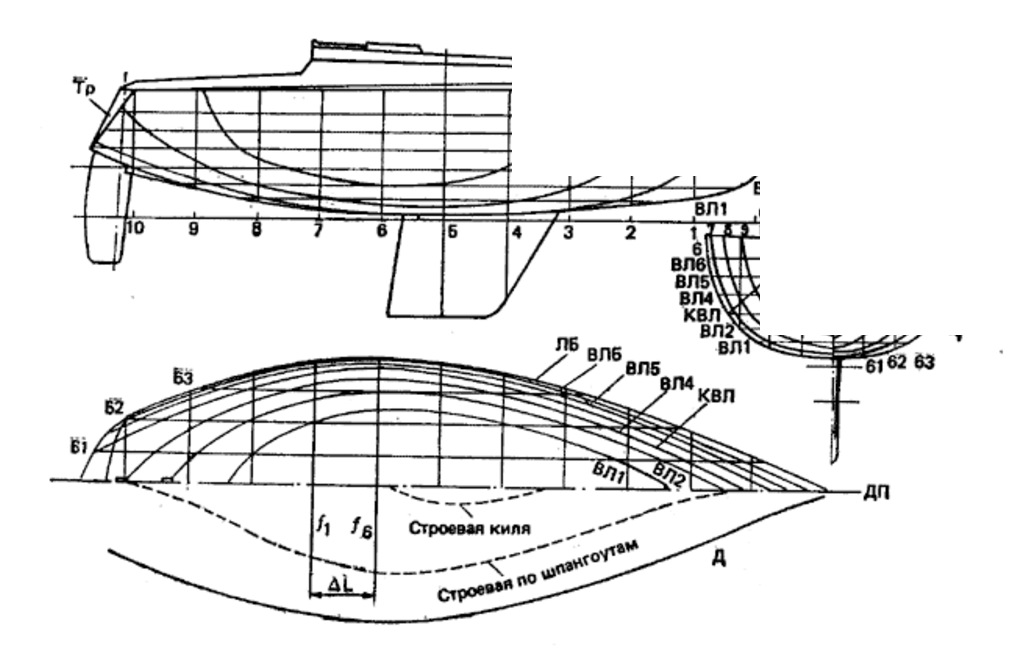
\includegraphics{pics/0002_Teor_chertezh}
   \caption{Теоретический чертеж яхты <<Симфония>>}
   \label{fig:2}
   \centering{}\small  1~--~10~---~шпангоуты, Тр~---~транец, ЛБ~---~линия борта, Б1~--~Б3~---~батоксы, ВЛ1~--~ВЛ6~---~ватерлинии, Д~---~диагональ, или рыбина).
\end{figure}

На теоретическом чертеже кроме упомянутых линий батоксов, шпангоутов и ватерлиний изображают очертания плавниковых килей, рулей, транца, фальшборта и т.~п. Так как корпус симметричен относительно \textit{ДП}, то на полушироте изображают ватерлинии только левого борта; на проекции <<Бок>> по правую сторону от линии \textit{ДП} вычерчивают обводы носовых шпангоутов, а по левую \--- обводы кормовых.

Все линии теоретического чертежа должны быть согласованы. Это значит, что любая точка на поверхности корпуса должна отстоять на равных расстояниях, например от \textit{ДП} на всех трех проекциях. При согласовании линий конструктор обычно проверяет положение точек пересечения кривых линий с прямыми линиями сетки. Для дополнительного согласования обводов корпуса на теоретическом чертеже проводят рыбины или диагонали \--- следы сечения корпуса продольными, наклонными к \textit{ДП} плоскостями, проведенными через характерные точки на проекции <<корпус>> \--- скулу, вогнутость при киле и т.~п. Диагонали проводятся только на <<корпусе>>, в виде прямых линий, и на полушироте вниз от \textit{ДП}, где они имеют вид плавных кривых линий.

Опытному глазу каждая из линий теоретического чертежа может многое сказать о качествах судна. Например, плавные стройные ватерлинии с острым входом в носу и не слишком крутой кривизной в корме благоприятны для хорошего обтекания корпуса водой, как и диагонали аналогичного вида. Батоксы с плавным и пологим \--- под углом $15\div20^\circ$ к \textit{КВЛ} выходом над ватерлинией также важны для плавного, без завихрений, обтекания корпуса. Шпангоуты с явно выраженной скулой и переходом днища в борта по малому радиусу свидетельствуют о высокой начальной остойчивости яхты. В носовой части V-образные шпангоуты с острой вершиной при киле и плавным расширением к палубе важны для сохранения скорости на взволнованном море и незаливаемости палубы. 

Существенное влияние на обводы корпуса оказывают \textbf{Правила обмера}, по которым строится яхта. Так, в 70-х годах в результате введенного в правила обмера IOR, замера глубины трюма (расстояний от \textit{КВЛ} до внутренней поверхности обшивки) на миделе в трех местах по ширине яхты появились суда с трапециевидными шпангоутами. Эти же Правила дали жизнь принципиально новым обводам корпусов \--- с короткими свесами оконечностей, <<обратным>> наклоном транца, высоким надводным бортом и плавниковым килем, которые значительно отличаются от классических яхтенных обводов, господствовавших до конца 60-х годов.

Важнейшей характеристикой яхты является ее \textbf{объемное водоизмещение} $V$, т. е. объем воды, вытесняемый яхтой при ее погружении по \textit{КВЛ}. Объемное водоизмещение яхты вместе с ее главными размерениями позволяет судить о величине судна, его вместимости и потенциальных мореходных качествах. При сравнении яхт часто пользуются безразмерной характеристикой \--- \textbf{коэффициентом полноты водоизмещения} или \textbf{коэффициентом общей полноты} $\delta$, связывающим линейные размеры корпуса с его погруженным объемом. Этот коэффициент определяется как отношение объемного водоизмещения к объему параллелепипеда, имеющего стороны, равные $L_{\mbox{квл}}$, $B_{\mbox{квл}}$ и $T_{\mbox{ср}}$ (рис.~\ref{fig:3}): $\delta = V/(L_{\mbox{квл}} \cdot B_{\mbox{квл}} \cdot  T_{\mbox{ср}})$.

\begin{figure}[htbp]
   \centering
   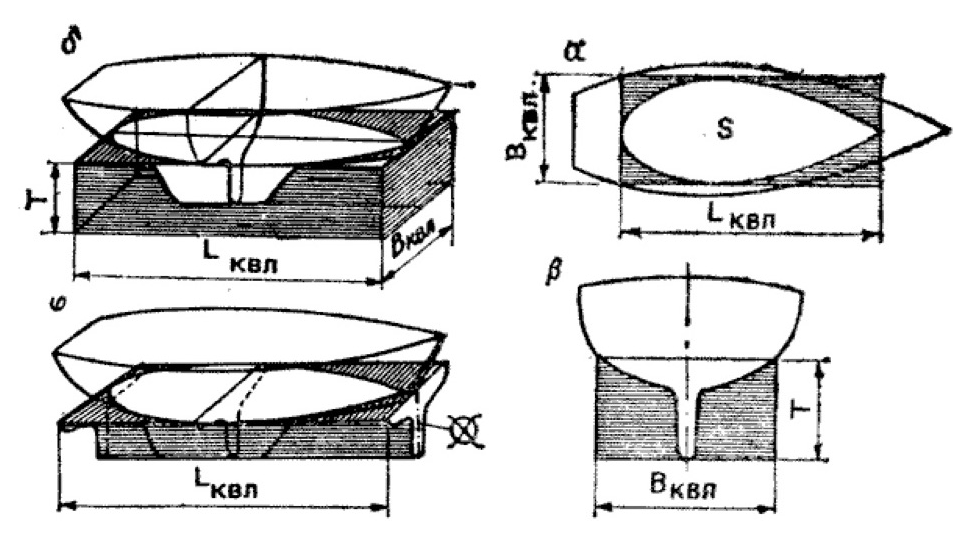
\includegraphics{pics/0003_Koeff_polnoty}
   \caption{Коэффициенты полноты}
   \label{fig:3}
   \centering{}\small $\delta$~---~водоизмещения; $\alpha$~---~ватерлинии; $\varphi$~---~продольной полноты; $\beta$~---~полноты мидель-шпангоута
\end{figure}

Чем меньше коэффициент общей полноты, тем более острые обводы имеет яхта, тем она быстроходнее. С другой стороны, при уменьшении $\delta$ соответственно уменьшается и полезный объем корпуса ниже ватерлинии, что вызывает необходимость для размещения кают достаточной высоты увеличивать высоту борта или делать более высокие надстройки. Парусные яхты относят к наименее полным судам. Коэффициент общей полноты для крейсерско-гоночных яхт составляет $\delta = 0.15 \div 0.22$, для крейсерских швертботов $\delta = 0.26 \div 0.35$. Корпуса шхерных крейсеров имели $\delta = 0.12 \div 0.15$, в то время как для большинства грузовых коммерческих судов характерна величина $\delta = 0.82$. 

\chapter{Правила обмера крейсерско-гоночных яхт}\label{chap:4}



\end{document}
